% VUT FIT MITAI
% MSZ 2021/2022
% Author: Vladimir Dusek
% Login: xdusek27

%%%%%%%%%%%%%%%%%%%%%%%%%%%%%%%%%%%%%%%%%%%%%%%%%%%%%%%%%%%%%%%%%%%%%%%%%%%%%%%%

% Path to figures
\graphicspath{{pds/prepinace/figures}}

%%%%%%%%%%%%%%%%%%%%%%%%%%%%%%%%%%%%%%%%%%%%%%%%%%%%%%%%%%%%%%%%%%%%%%%%%%%%%%%%

\chapter{PDS~--~Základní architektury přepínačů, algoritmy pro plánování, řešení blokování, vícestupňové přepínací sítě.}

% Ohledne CAM tabulky:
% Útoky v počítačových sítích, zaměřit se na L2 vrstvu (CAM, ARP, ...): chtěl nejdříve popsat co je to switch, k čemu je (přepínání packetů na L2), pak popsat CAM tabulku, co v ní najdeme (MAC, Port, VLAN), jak se CAM tabulka tvoří (tady jsem to trochu domotal ale nakonec jsme se nějak shodli - switch prohlíží L2 hlavičky příchozích packetů, které přes něj prochází, a podle toho si tvoří záznamy v tabulce) - na example topologii ukázat co je to CAM overflow a jak jej útočník způsobí (generuje packety s různými MAC adresami a posílá je do sítě, aby naplnil CAM tabulku nepoužitelnými záznamy), k čemu to vede (switch začne broadcastovat packety, které pak útočník může odposlouchávat). Vzhledem k tomu, jak jsem zmatkoval při popisu CAM tabulky a její tvorby se asi rozhodl, že dál se ptát raději nebude + už odzvonil budík.

%%%%%%%%%%%%%%%%%%%%%%%%%%%%%%%%%%%%%%%%%%%%%%%%%%%%%%%%%%%%%%%%%%%%%%%%%%%%%%%%

\section{Metadata}

\begin{compactitem}
    \item Předmět: Přenos dat, počítačové sítě a protokoly (PDS)
    \item Přednáška:
    \begin{compactitem}
        \item \path{04-switching.pdf}
    \end{compactitem}
    \item Záznam:
    \begin{compactitem}
        \item 2021-03-05
    \end{compactitem}
\end{compactitem}

%%%%%%%%%%%%%%%%%%%%%%%%%%%%%%%%%%%%%%%%%%%%%%%%%%%%%%%%%%%%%%%%%%%%%%%%%%%%%%%%

\section{Úvod a kontext}

% Todo:
% - prepinace nemodifikuji paket
% - prepinace samy o sobe nepotrebuji MAC adresu a vetsinou nemaji zadnou
% - "The basic function of a switch is transparent bridging" - preposle paket a nikdo to ani nepozna

\paragraph*{ISO/OSI model} Referenční model ISO/OSI se používá jako názorný příklad řešení komunikace v počítačových sítích pomocí vrstevnatého modelu, kde jsou jednotlivé vrstvy nezávislé a snadno nahraditelné. \begin{compactitem}

    \item \textbf{Aplikační vrstva} (L7, \textit{application layer}) \begin{compactitem}
        \item Zajišťuje zpracování dat na nejvyšší úrovni (reprezentace dat, kódování, řízení dialogu, \dots).
        \item Tvořena procesy a aplikacemi, které komunikují po síti.
        \item Bývá slučována s prezentační vrstvou (L6, prezentace dat a šifrování) a relační vrstvou (L5, koordinace a komunikace).
        \item Příklad protokolů: \begin{compactitem}
            \item Uživatelské~--~vykonávají služby přímo uživateli (Telnet, SSH, FTP, SMTP, HTTP, \dots)
            \item Systémové~--~zajišťují síťové funkce (DNS, DHCP, SNMP, BOOTP, \dots)
        \end{compactitem}
    \end{compactitem}

    \item \textbf{Transportní vrstva} (L4, \textit{transport layer}) \begin{compactitem}
        \item Rozděluje aplikační data (segmentace) na menší jednotky a zapouzdřuje je do segmentů (TCP) / datagramů (UDP).
        \item Vytváří logické spojení mezi procesy (přenáší data konkrétní aplikace ze zdrojového zařízení do aplikace na cílovém zařízení).
        \item Adresace: porty.
        \item Příklad protokolů: TCP, UDP, DCCP, SCTP, MP-TCP, QUIC
    \end{compactitem}

    \item \textbf{Síťová vrstva} (L3, \textit{network layer}) \begin{compactitem}
        \item Zapouzdřuje segmenty/datagramy do paketů.
        \item Řeší směrování.
        \item Adresace: IP adresa (logická adresa).
        \item Příklad protokolů: IPv4, IPv6, ARP, RARP, ICMP,IGMP
    \end{compactitem}

    \item \textbf{Linková vrstva} (L2, \textit{data link layer}, vrstva síťového rozhraní, \textit{network interface layer}) \begin{compactitem}
        \item Zapouzdřuje pakety do rámců.
        \item Zajišťuje \textit{hop-by-hop} doručení.
        \item Adresace: MAC adresa (fyzická adresace).
        \item Příklad protokolů: Ethernet, Token Ring, FDDI, X.25, Frame Relay
    \end{compactitem}

    \item \textbf{Fyzická vrstva} (L1, \textit{physical layer}) \begin{compactitem}
        \item Zajišťuje přenos bitů přes fyzické médium.
    \end{compactitem}

\end{compactitem}

\paragraph*{data, segment, datagram, paket, rámec, bit} \begin{compactitem}
    \item Data~--~aplikační vrstva (L7)
    \item Segment~--~transportní vrstva (L4), TCP
    \item Datagram~--~transportní vrstva (L4), UDP
    \item Paket~--~síťová vrstva (L3)
    \item Rámec~--~linková vrstva (L2)
    \item Bit~--~fyzická vrstva (L1)
\end{compactitem}

\paragraph*{CAM tabulka} CAM tabulka je datová struktura v přepínači, která uchovává informace o tom, za jakým fyzickým portem je zařízení s jakou MAC adresou. Jak se plní? Přepínač si ji plní automaticky. V momentě kdy k němu přijde paket, doplní si MAC adresu a port přes který paket přišel. Pokud přepínač neví za jakým portem je cílová MAC adresa, pošle to všem (\textit{flooding}).

\paragraph*{Propustnost} Kolik je možné přenést dat za časovou jednotku.

% src: https://linuxhint.com/network-osi-layers-explained
\begin{figure}[H]
    \centering
    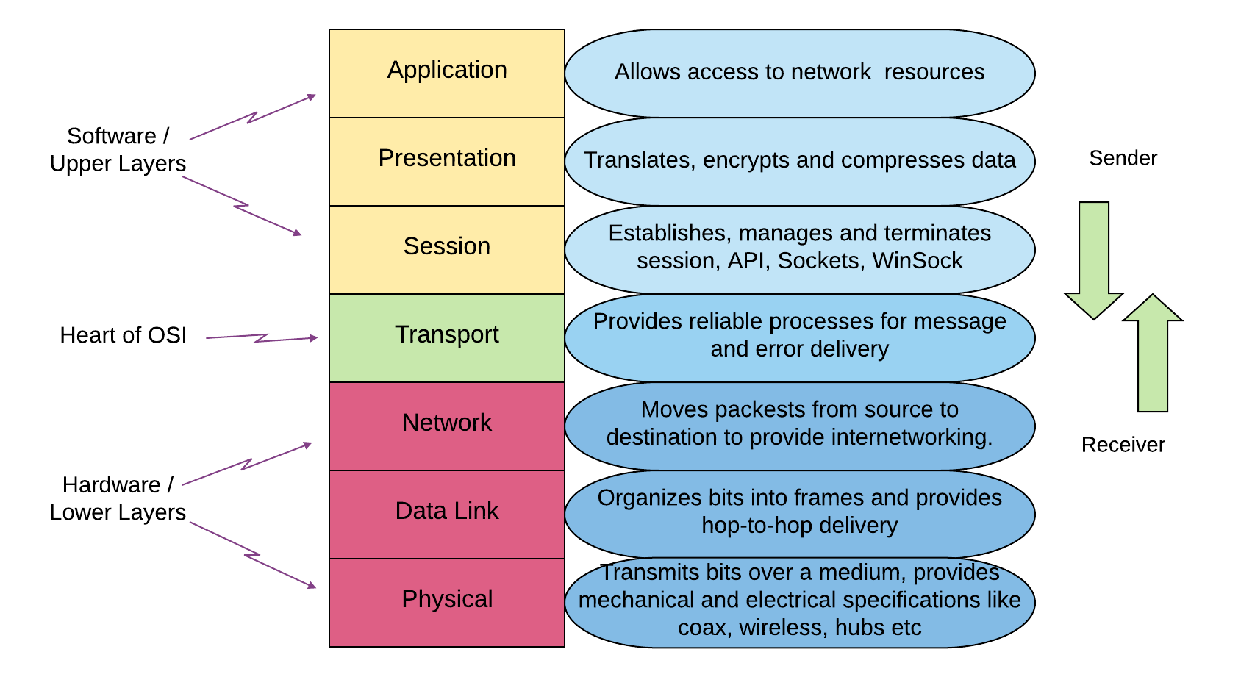
\includegraphics[width=1\linewidth]{osi_model_linuxhint.pdf}
    \caption{Příklad OSI modelu z Linuxhint.}
\end{figure}

% src: https://cs.wikipedia.org/wiki/Soubor:OSI_Model_v1.svg
\begin{figure}[H]
    \centering
    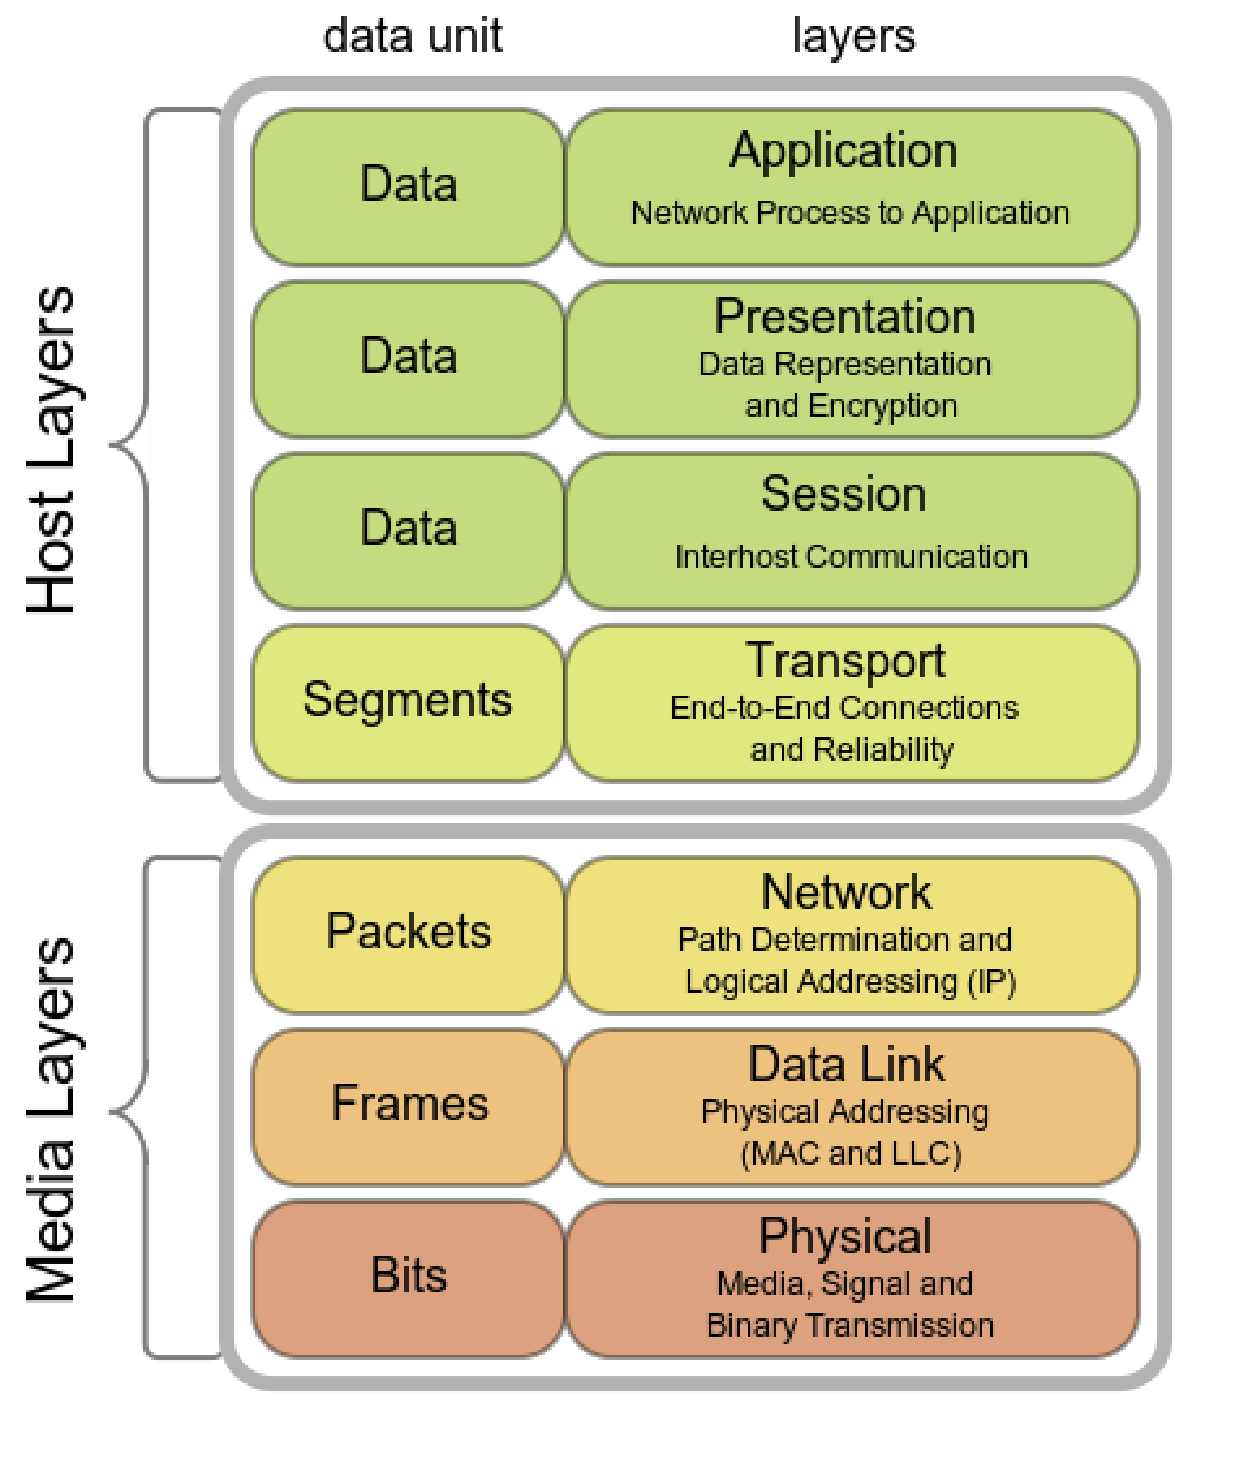
\includegraphics[width=0.65\linewidth]{osi_model_wiki.pdf}
    \caption{Příklad OSI modelu z Wiki.}
\end{figure}

%%%%%%%%%%%%%%%%%%%%%%%%%%%%%%%%%%%%%%%%%%%%%%%%%%%%%%%%%%%%%%%%%%%%%%%%%%%%%%%%

\section{Obecná architektura přepínače}

Síťový přepínač (\textit{switch}) je aktivní prvek v počítačové síti, který propojuje jednotlivé prvky do hvězdicové topologie. Přepínač obsahuje síťové porty (až stovky), na něž se připojují síťová zařízení. \begin{compactitem}
    \item Na jaké vrstvě OSI modelu pracuje? Pracuje s rámci (linková vrstva, L2).
    \item Na základě čeho provádí přepínání? Na základě cílové MAC adresy.
    \item Jaké typy přenosů přepíná? Na základě cílové MAC adresy rozslišuje typ přenosu: \begin{compactitem}
        \item broadcast (samé 1),
        \item multicast (speciální prefix pro IPv4 a IPv6),
        \item unicast (cokoliv jiného).
    \end{compactitem}
    \item Co ovlivňuje rychlost přepínání? \begin{compactitem}
        \item Hardware (typ paměti, rychlost procesoru)
        \item Logika přepínání
        \item Šířka pásma cílového rozhraní
    \end{compactitem}
\end{compactitem}

\paragraph*{Požadavky na přenos} \begin{compactitem}
    \item Maximální využití sběrnice (požadavek na plánovač). \begin{compactitem}
        \item Aby došlo k maximálnímu přenosu dat přepínací logikou (co nejvíce přenosů v rámci taktu~--~\uv{paralelizace}).
    \end{compactitem}
    \item Spravedlivé přidělování přenosového pásma (aby byly obsluhovány všechny porty).
    \item Zachování pořadí rámců (ne vždy je možné).
\end{compactitem}

\begin{figure}[H]
    \centering
    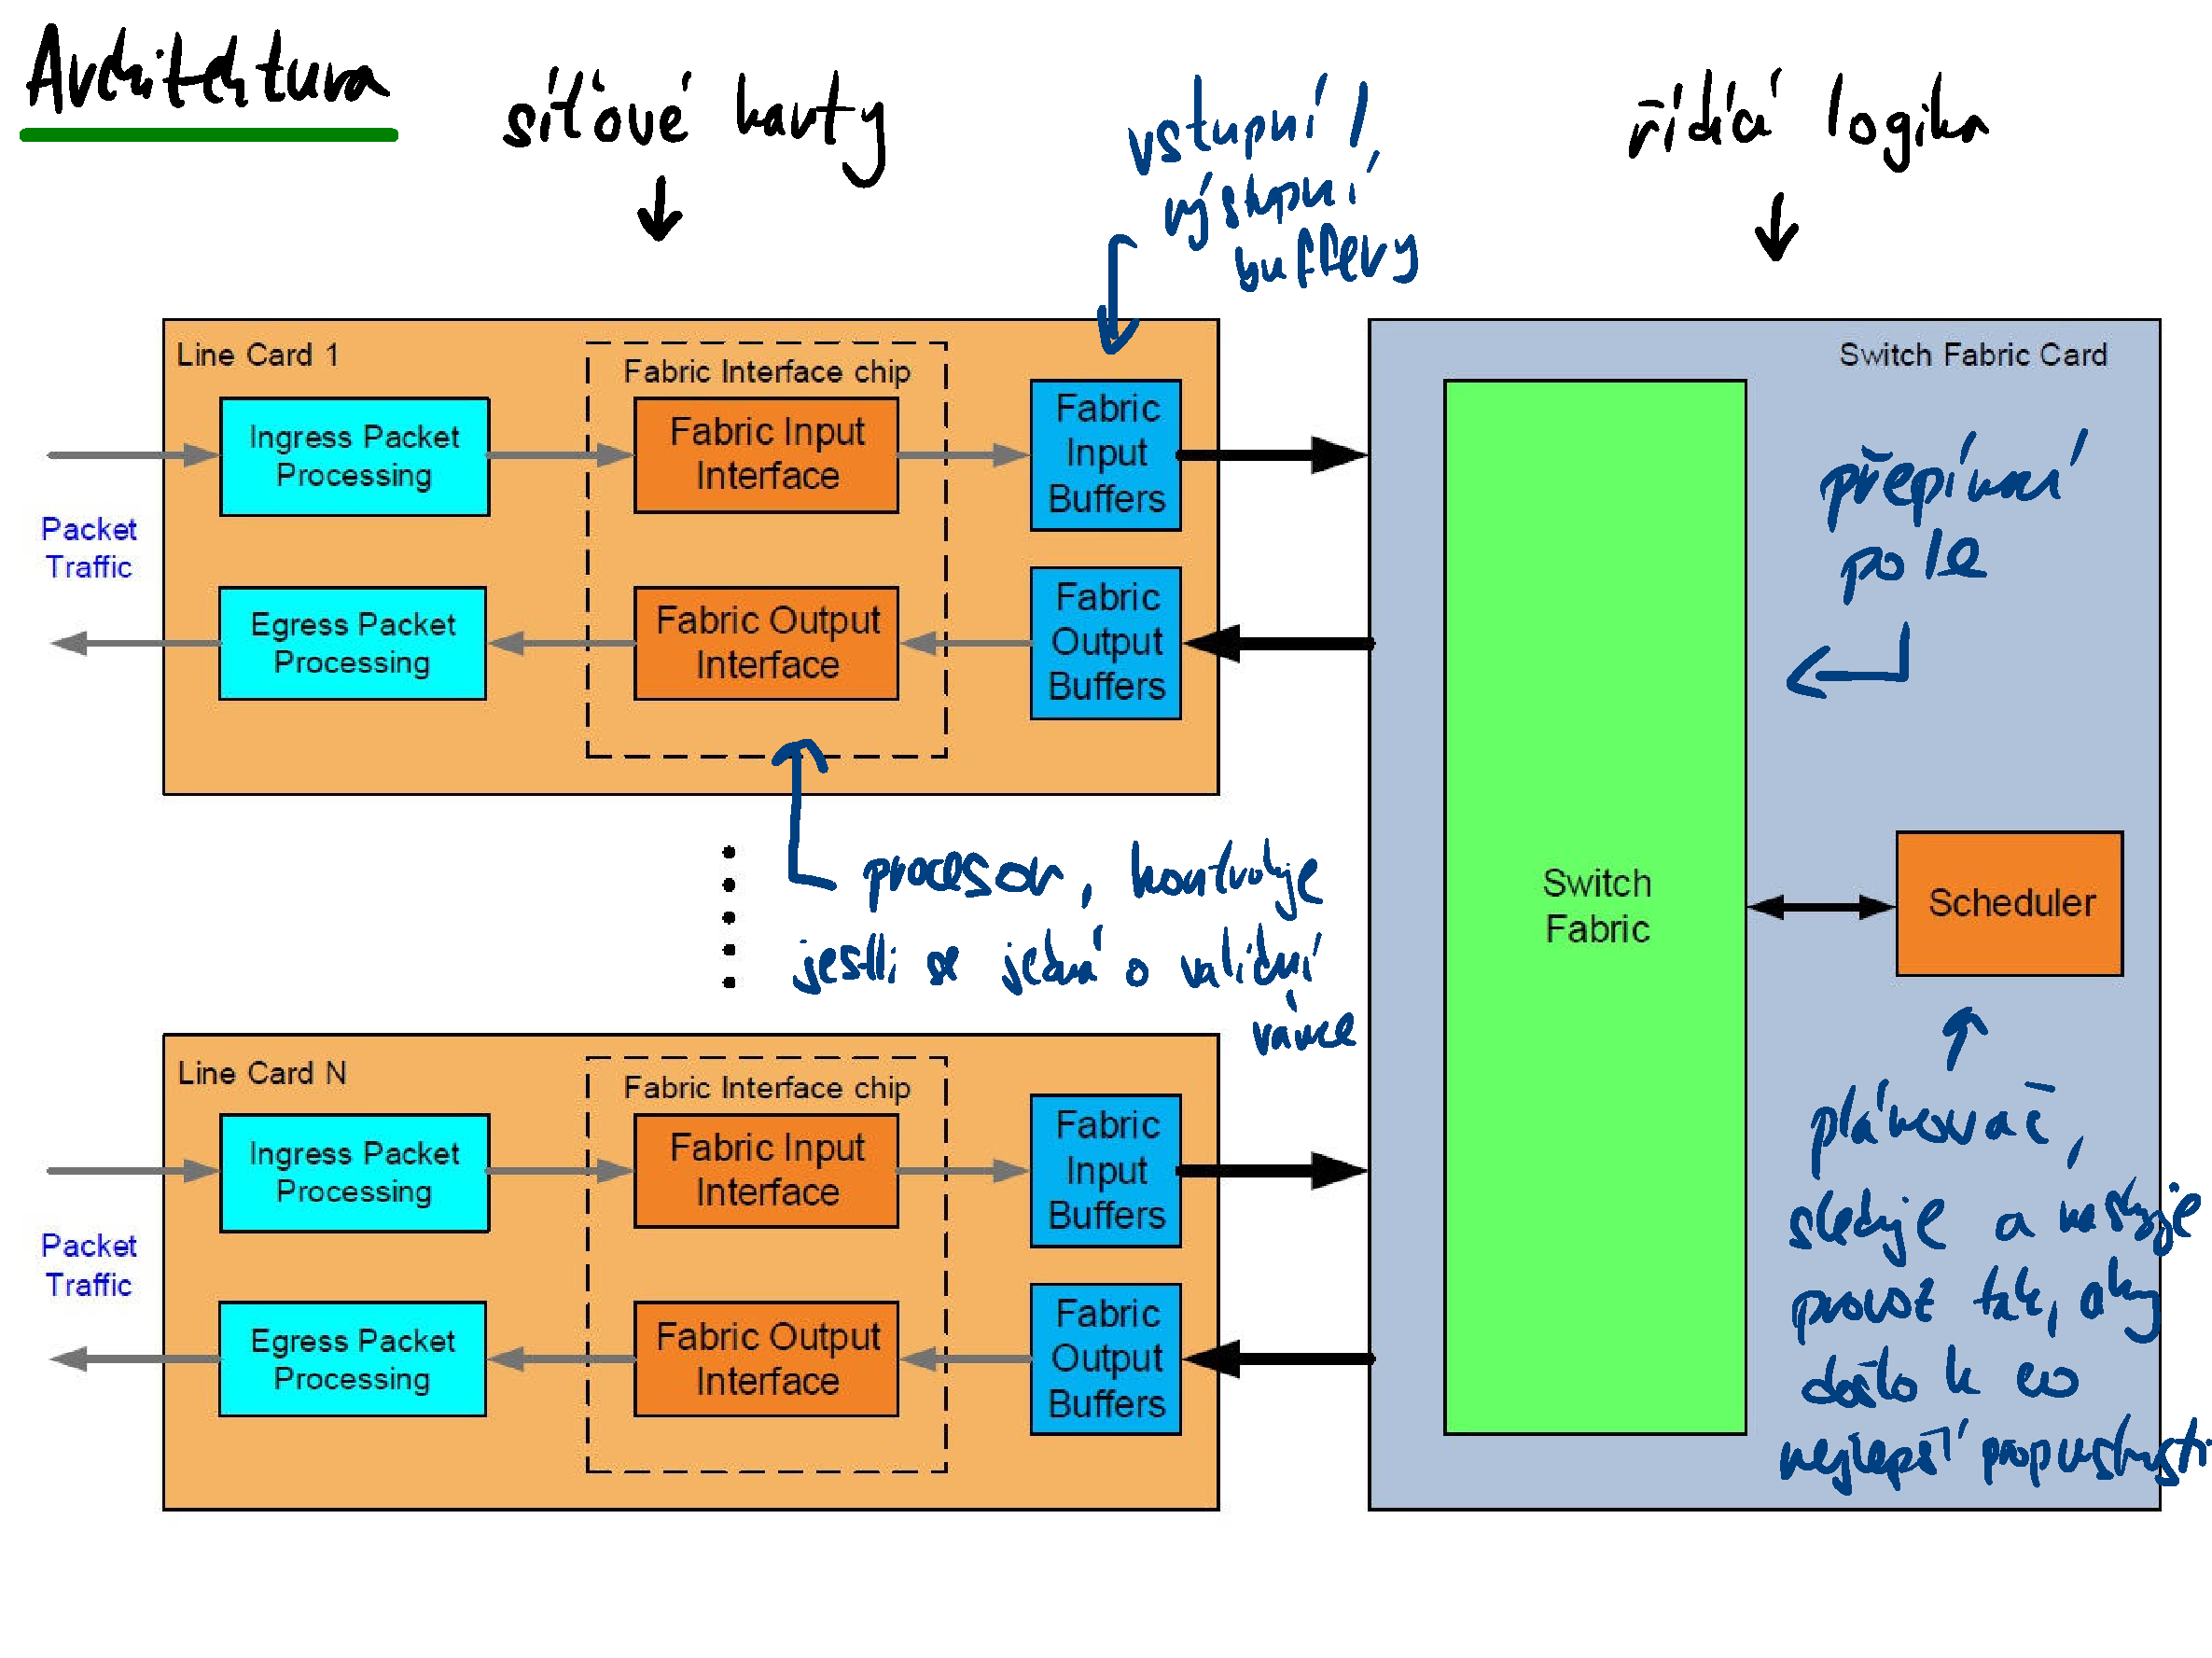
\includegraphics[width=1\linewidth]{obecna_architektura.pdf}
    \caption{Obecná architektura přepínače.}
    \label{pds_obecna_architektura_prepinace}
\end{figure}

\begin{figure}[H]
    \centering
    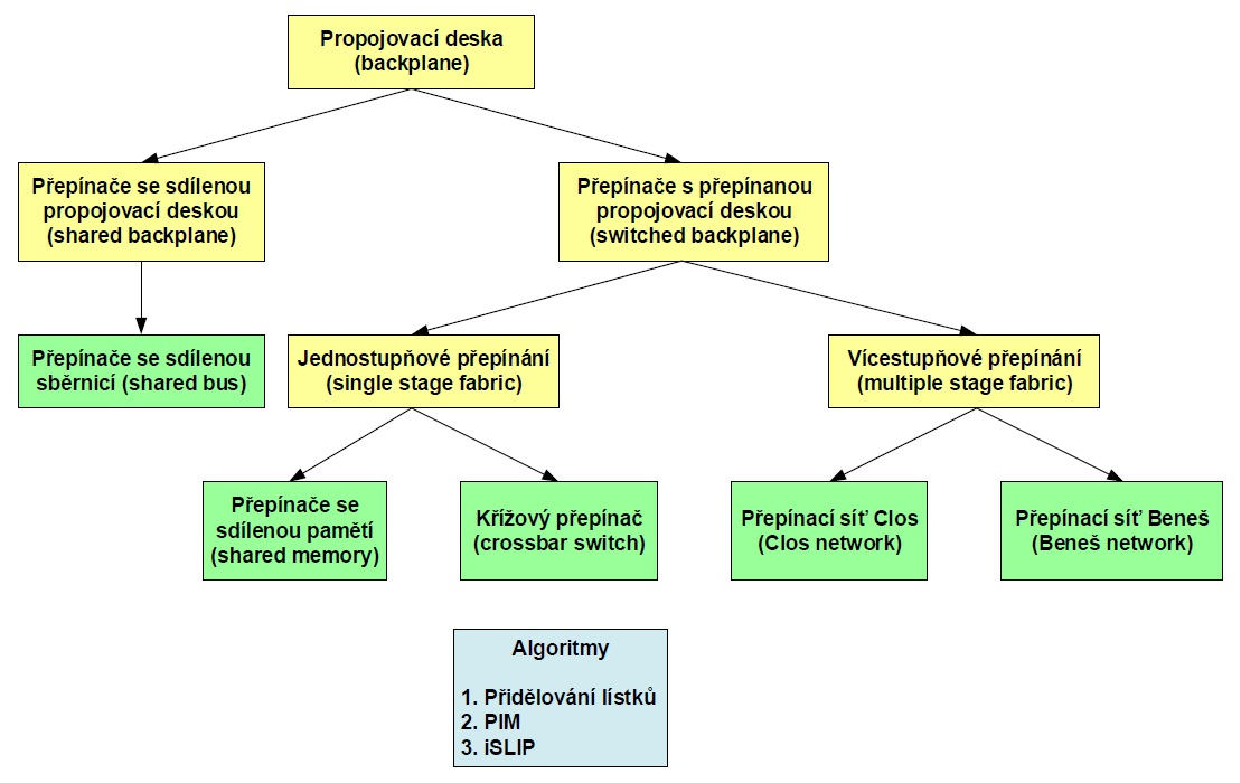
\includegraphics[width=1\linewidth]{deleni_prepinacu.pdf}
    \caption{Dělení přepínačů.}
\end{figure}

% \paragraph*{Dělení přepínačů} \begin{compactitem}
%     \item Přepínače se sdílenou propojovací deskou (\textit{shared backplane}) \begin{compactitem}
%         \item Přepínače se sdílenou sběrnicí (\textit{shared bus})
%     \end{compactitem}
%     \item Přepínače s přepínanou propojovací deskou (\textit{switched backplane}) \begin{compactitem}
%         \item Jednostupňové přepínání (\textit{single stage fabric}) \begin{compactitem}
%             \item Přepínače se sdílenou pamětí (\textit{shared memory})
%             \item Křížový přepínač (\textit{crossbar switch}) \begin{compactitem}
%                 \item Algoritmus přidělování lístků
%                 \item Algoritmus PIM
%                 \item Algoritmus iSLIP
%             \end{compactitem}
%         \end{compactitem}
%         \item Vícestupňové přepínání \begin{compactitem}
%             \item Přepínací síť Clos
%             \item Přepínací síť Beneš
%         \end{compactitem}
%     \end{compactitem}
% \end{compactitem}

%%%%%%%%%%%%%%%%%%%%%%%%%%%%%%%%%%%%%%%%%%%%%%%%%%%%%%%%%%%%%%%%%%%%%%%%%%%%%%%%

\section{Přepínače se sdílenou propojovací deskou}

\subsection{Přepínače se sdílenou sběrnicí}

\begin{compactitem}
    \item Může komunikovat pouze jeden port v daný čas, ostatní čekají (řízeno protokolem).
    \item Lze jednoduše realizovat broadcast a multicast.
    \item Mějme $N$ portů (karet), rychlost každé karty $R$ bps, taktovací frekvenci $r$. Pak rychlost sběrnice musí být $N \times R$ a šířka sběrnice $$W = \frac{R \times N}{r}$$
    \item Pokud se přidají nové porty nebo se na nich zvýší rychlost je potřeba zvýšit propustnost sběrnice (\uv{něco za něco}).
\end{compactitem}

\begin{figure}[H]
    \centering
    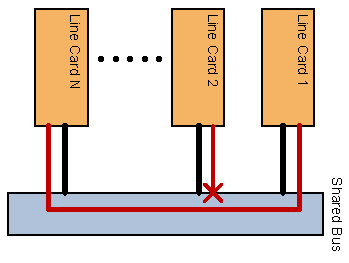
\includegraphics[width=0.5\linewidth]{sdilena_deska_sdilena_sbernice.pdf}
    \caption{Přepínač se sdílenou sběrnicí.}
\end{figure}

\begin{figure}[H]
    \centering
    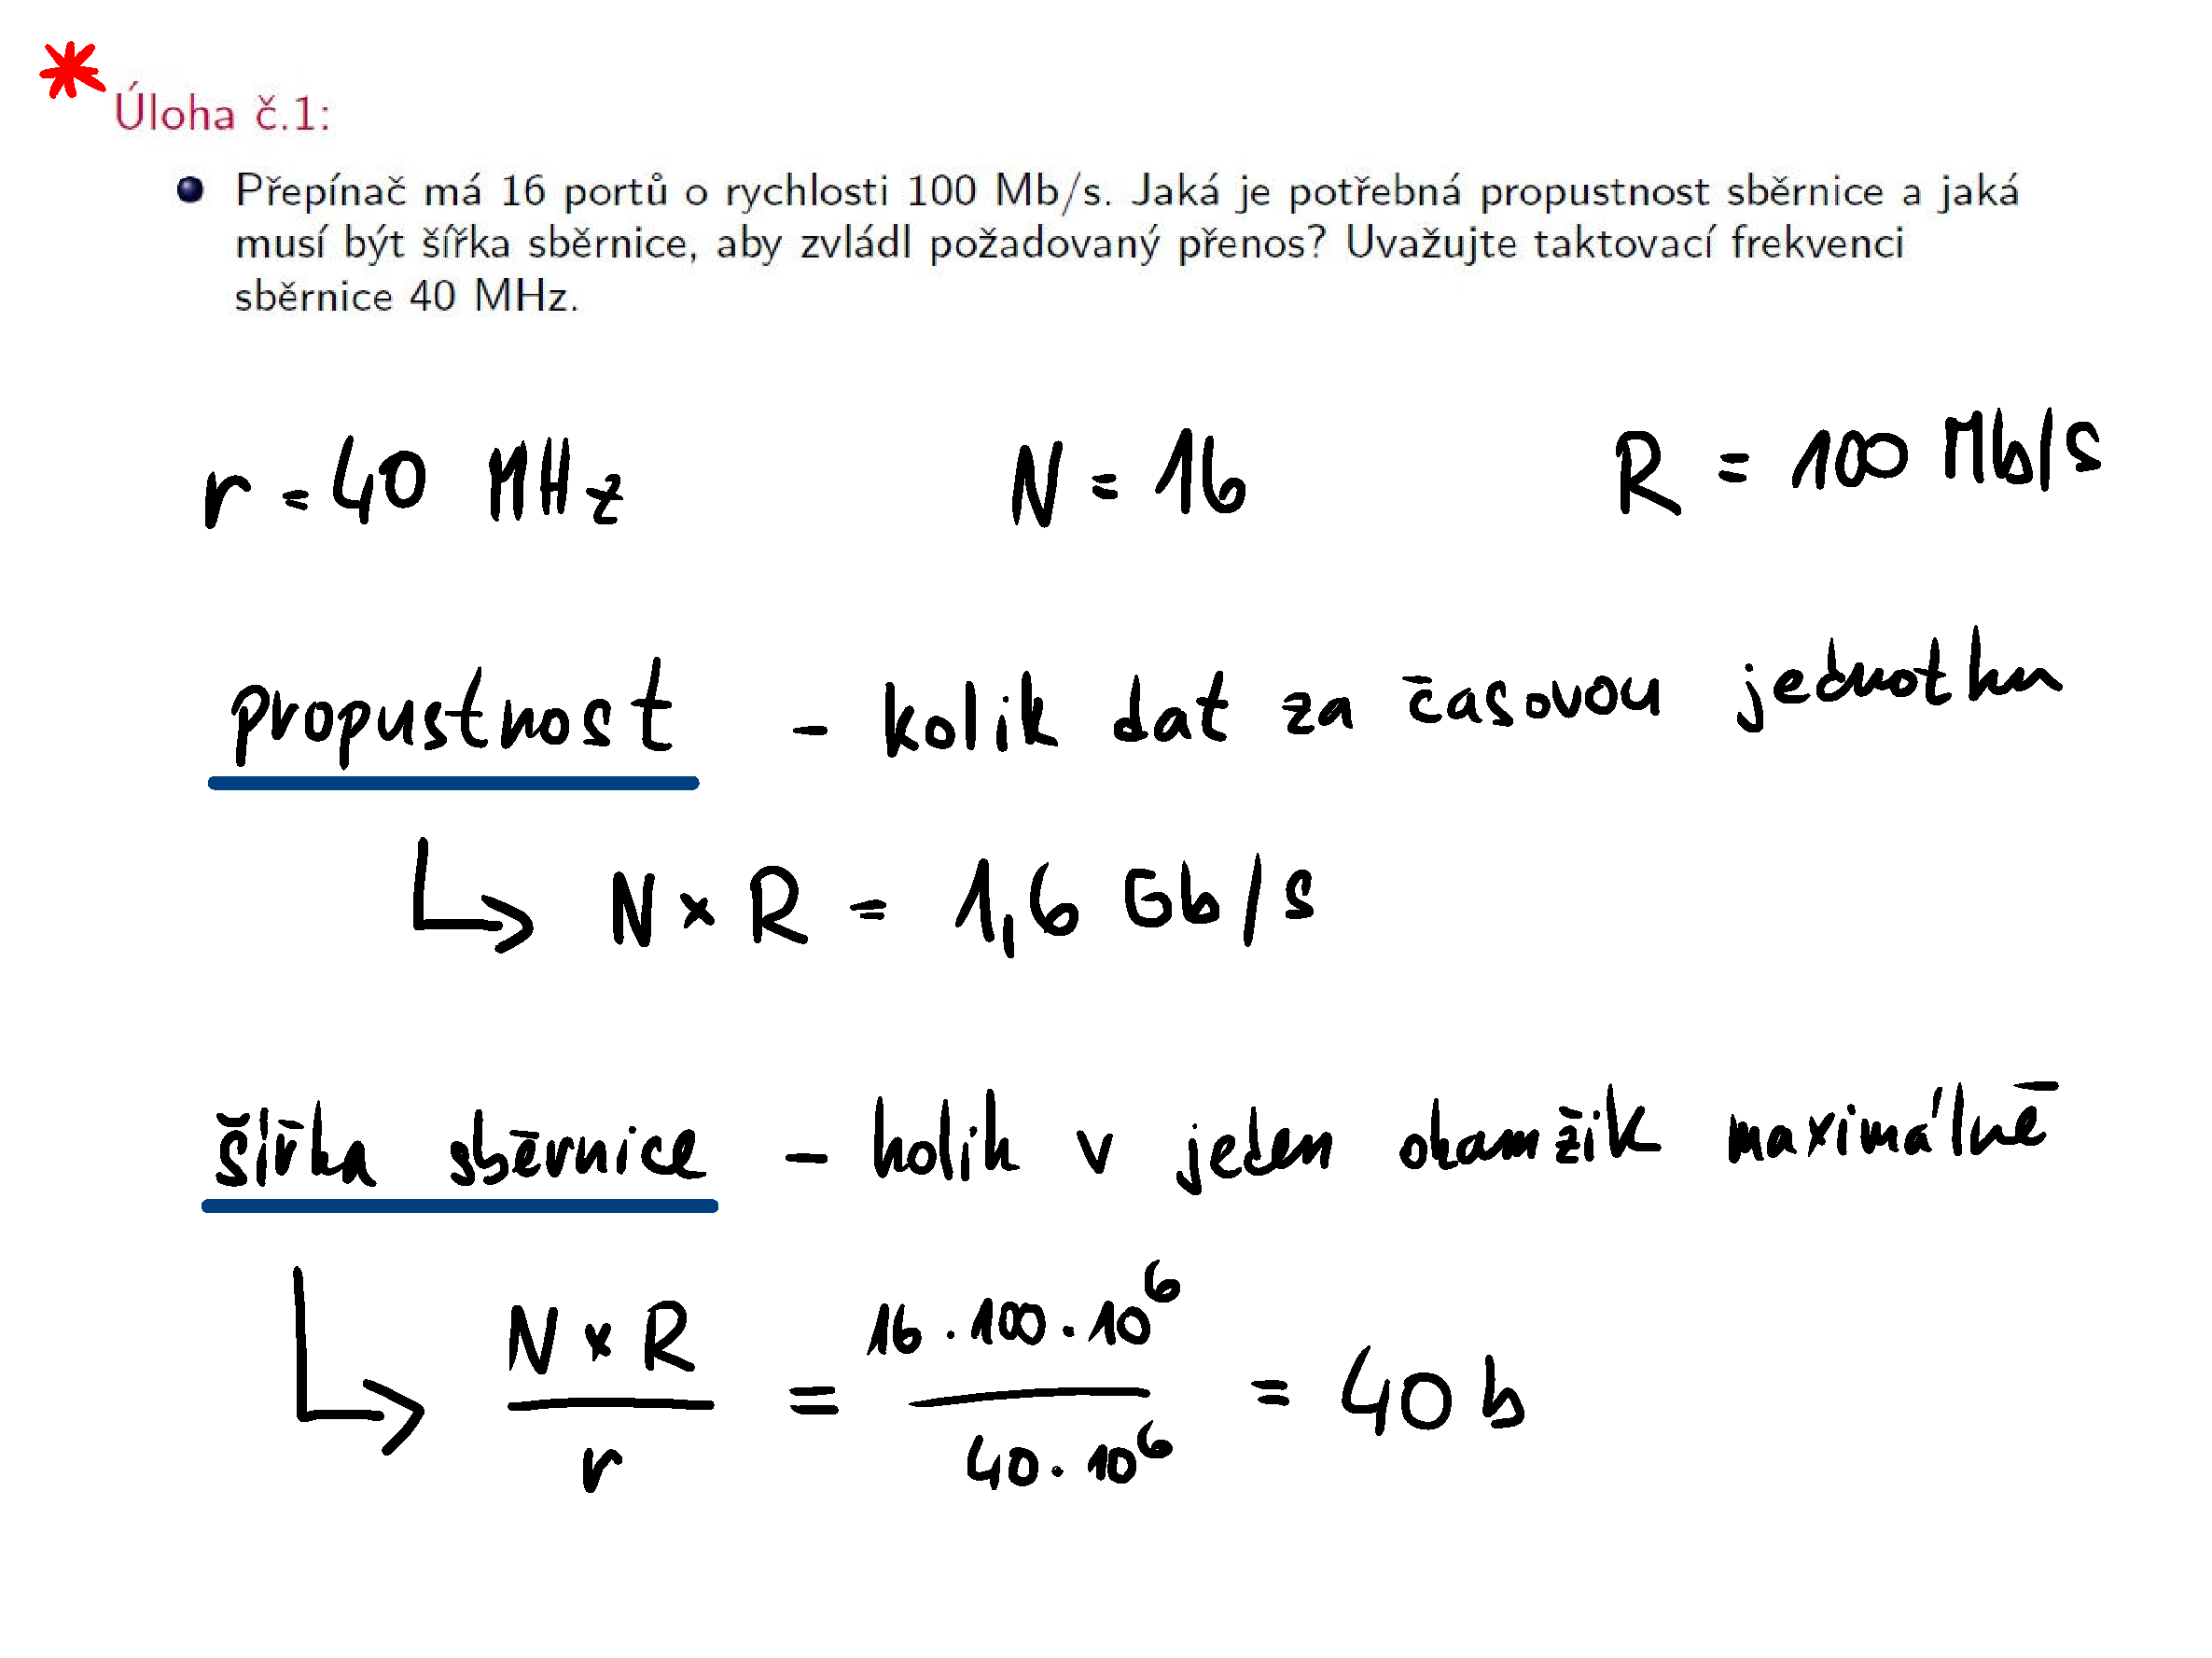
\includegraphics[width=1\linewidth]{sdilena_deska_sdilena_sbernice_priklad.pdf}
    \caption{Přepínač se sdílenou sběrnicí~--~příklad.}
\end{figure}

%%%%%%%%%%%%%%%%%%%%%%%%%%%%%%%%%%%%%%%%%%%%%%%%%%%%%%%%%%%%%%%%%%%%%%%%%%%%%%%%

\section{Přepínače s přepínanou propojovací deskou: jednostupňové přepínání}

\begin{compactitem}
    \item Umožňuje paralelní přenos rámců.
    \item Je potřeba plánovač (\textit{scheduler}), který plánuje přenos.
    \item Provedení přenosu: z bufferů vstupních karet se data přenesou do bufferů výstupních karet.
\end{compactitem}

\begin{figure}[H]
    \centering
    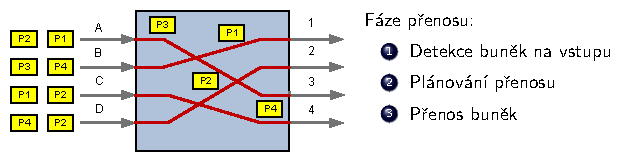
\includegraphics[width=1\linewidth]{prepinana_propojovaci_deska.pdf}
    \caption{Činnost přepínače s přepínanou propojovací deskou.}
\end{figure}

\subsection{Přepínače se sdílenou pamětí}

\begin{compactitem}
    \item Centrální sdílená paměť, která obsahuje frontu pro každý výstupní buffer (každý port).
    \item Pro jeden přenos se musí 2x přistoupit do paměti (zápis a čtení).
    \item Zde narážíme na současné technologické limity pamětí (rychlost přístupu).
\end{compactitem}

\begin{figure}[H]
    \centering
    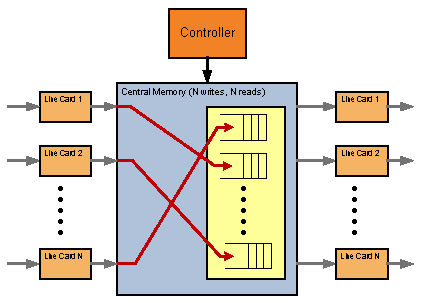
\includegraphics[width=1\linewidth]{prepinana_deska_sdilena_pamet.pdf}
    \caption{Činnost přepínače s přepínanou propojovací deskou a se sdílenou pamětí. Obsahuje: $N$ vstupních karet, řadič, sdílenou paměť s $N$ frontami, $N$ výstupních karet.}
\end{figure}

\begin{compactitem}
    \item Nechť $R$ je rychlost síťové kart, $N$ je počet síťových karet, pak celková propustnost přepínače je $BW = 2 \times N \times R$ (dva přístupy do paměti).
    \item Mějme data o velikosti $C$, pak doba přenosu je $t = C \div BW [s]$.
\end{compactitem}

\begin{figure}[H]
    \centering
    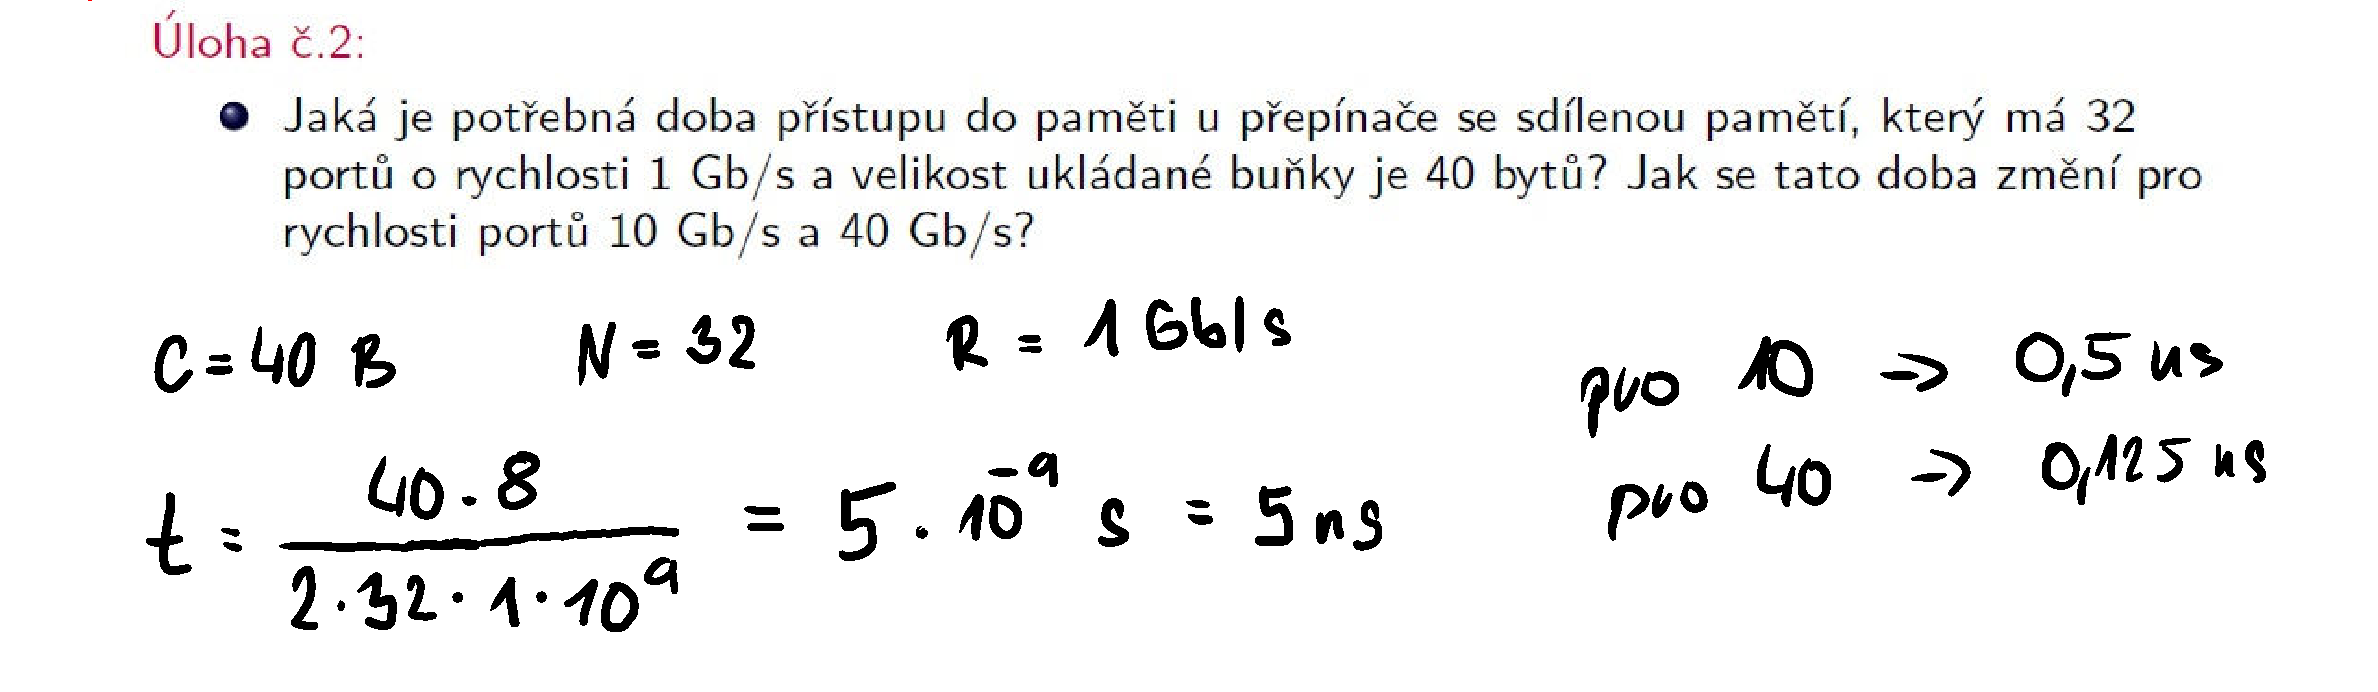
\includegraphics[width=1\linewidth]{prepinana_deska_sdilena_pamet_priklad.pdf}
    \caption{Přepínač s přepínanou sběrnicí a se sdílenou pamětí~--~příklad.}
\end{figure}

\subsection{Křížové přepínače (\textit{crossbar})}

\begin{compactitem}
    \item Založený na jednom velkém propojovacím poli.
    \item Interně neblokující.
    \item Nativní podpora multicastu.
    \item Je potřeba $N^2$ propojení.
    \item Chybí redundance: pouze jedna cesta mezi vstupem a výstupem.
\end{compactitem}

\begin{figure}[H]
    \centering
    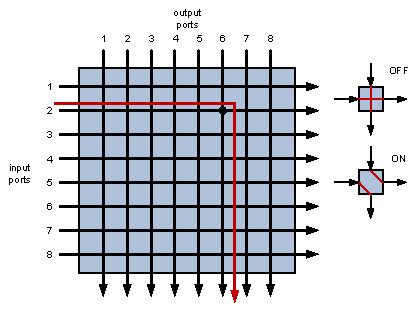
\includegraphics[width=0.75\linewidth]{prepinana_deska_krizovy.pdf}
    \caption{Přepínač s přepínanou sběrnicí a křížovými propoji.}
\end{figure}

%%%%%%%%%%%%%%%%%%%%%%%%%%%%%%%%%%%%%%%%%%%%%%%%%%%%%%%%%%%%%%%%%%%%%%%%%%%%%%%%

\section{Hledání spojů v křížovém přepínači}

\subsection{Problém párování}

V kontextu přepínání v křížovém přepínači se jedná o problém párování v bipartitním grafu, kde množina vstupních portů je $V_1$, množina výstupních portů je $V_2$ a hrany $E$ jsou propoje vstupů a výstupů. Množina $M$ se nazývá párování, pokud $M \subseteq E$, kde žádné dvě hrany z M, nemají společný vrchol.

\paragraph*{Bipartitní graf} Nechť $G = (V, E)$ je graf. Graf G je bipartitní, pokud platí $V = V_1 \cup V_2 \, \land \, V_1 \cap V_2 = \emptyset \, \land \, \forall e = \{u, v\}, e \in E : u \in V_1 \, \land \, v \in V_2$. Platí li navíc $E = V_1 \times V_2$, pak je graf úplný bipartitní.

\paragraph*{Největší párování} Největší párování (\textit{maximum matching}) je párování, které má největší počet hran (globální maximum). Složitost: $O(N^{5/2})$.

\paragraph*{Maximální párování} Maximální párování (\textit{maximal matching}) je párování, kdy nelze přidat žádnou další hranu (lokální maximum). Složitost: $O(N+E)$.

\bigskip\noindent Jelikož algoritmy pro hledání maximálního párování mají výrazně menší časovou složitost, volíme pro hledání spojů v křížovém přepínači ty.

\subsection{Algoritmus přidělování lístků}

\begin{compactitem}
    \item Princip: \begin{compactitem}
        \item Výstupní port $Q$ obsluhuje frontu požadavků na propojení.
        \item Požadavek na vstupu $P$ dostane od $Q$ číslo $T_{QX}$ pro obsloužení portu $Q$ s pořadím $X$.
    \end{compactitem}
    \item Fáze: \begin{compactenum}
        \item Žádost o lístek
        \item Přidělení lístku
        \item Propojení vstupů s výstupy a přenos
    \end{compactenum}
    \item Hodnocení: \begin{compactitem}
        \item Umožňuje přenos rámců s proměnlivou délkou
        \item \textbf{Blokování na začátku fronty} (\textit{head of line blocking})~--~Situace, kdy více vstupů chce stejný výstup. Musí se zpracovat ve více kolech. Řešení: Virtuální výstupní fronty (každý vstupní port má frontu pro každý výstupní port). Tím může dojít k předbíhání rámců. Viz další algoritmy.
    \end{compactitem}
\end{compactitem}

\begin{figure}[H]
    \centering
    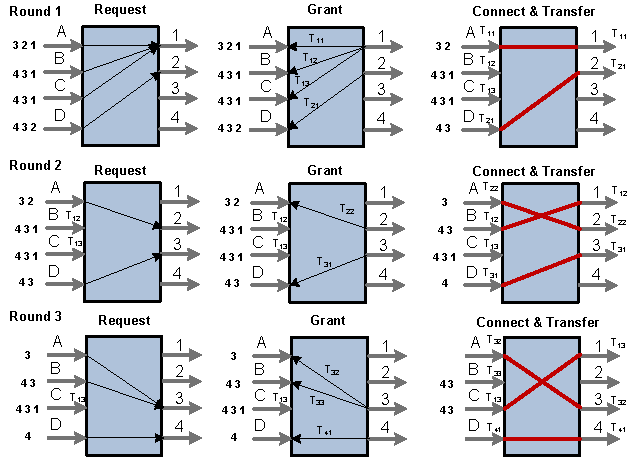
\includegraphics[width=1\linewidth]{algoritmus_pridelovani_listku_priklad.pdf}
    \caption{Příklad činnosti algoritmu přidělování lístků.}
\end{figure}

\subsection{Algoritmus PIM (\textit{Parallel Iterative Matching})}

\begin{compactitem}
    \item Algoritmus přidělování lístků + virtuální výstupní fronty + náhodnost. \begin{compactitem}
        \item Posílají se požadavky pro všechny pakety ve frontě, nikoliv pouze pro první.
    \end{compactitem}
    \item Hledá maximální párování (pomocí náhodné volby, která zabrání vyhladovění).
    \item Soutěžení o porty \begin{compactitem}
        \item Výstupní port~--~více žádostí naráz, jednu vyberu náhodně.
        \item Vstupní port~--~povolení na více výstupů naráz, jeden vyberu náhodně.
    \end{compactitem}
\end{compactitem}

\begin{figure}[H]
    \centering
    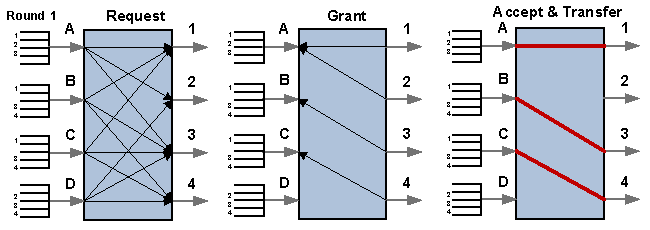
\includegraphics[width=1\linewidth]{algoritmus_pim_priklad_1.pdf}
    \caption{Příklad činnosti algoritmu PIM, kolo 1.}
\end{figure}

\begin{figure}[H]
    \centering
    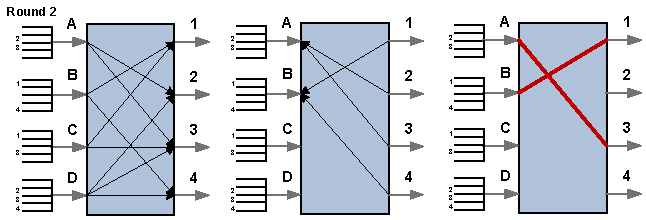
\includegraphics[width=1\linewidth]{algoritmus_pim_priklad_2.pdf}
    \caption{Příklad činnosti algoritmu PIM, kolo 2.}
\end{figure}

\begin{figure}[H]
    \centering
    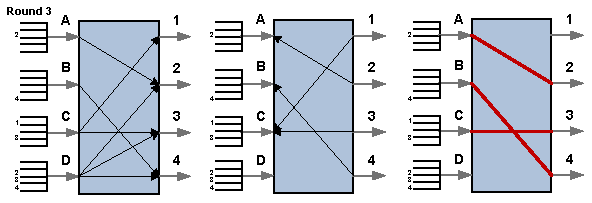
\includegraphics[width=1\linewidth]{algoritmus_pim_priklad_3.pdf}
    \caption{Příklad činnosti algoritmu PIM, kolo 3.}
\end{figure}

\subsection{Algoritmus iSLIP}

\begin{compactitem}
    \item Algoritmus přidělování lístků + virtuální výstupní fronty + iterace + ukazatele.
    \item Algoritmus \uv{rotujících ukazatelů} (vyhneme se náhodnému výběru). \begin{compactitem}
        \item Každý vstupní port má ukazatel (počítadlo), podle kterého se určuje priorita výstupu.
        \item Každý výstupní port má ukazatel, podle kterého se určuje priorita vstupu.
        \item Nová hodnota ukazatele je port na který se posílá / port od kterého se přijímá $+ 1$.
    \end{compactitem}
    \item Každé kolo má dvě iterace, resp. 6 fází~--~\textit{request}, \textit{grant}, \textit{accept}, \textit{request}, \textit{grant}, \textit{accept and transfer}. \begin{compactitem}
        \item Proč? Protože fáze \textit{transfer} trvá nejdéle (optimalizace).
    \end{compactitem}
\end{compactitem}

\begin{figure}[H]
    \centering
    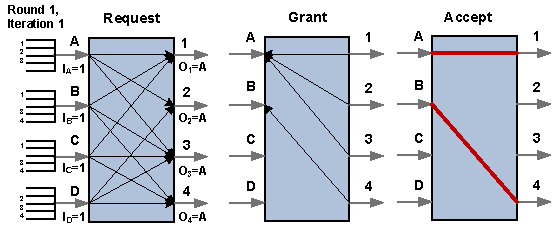
\includegraphics[width=1\linewidth]{algoritmus_islip_priklad_1.pdf}
    \caption{Příklad činnosti algoritmu iSLIP, kolo 1.}
\end{figure}

\begin{figure}[H]
    \centering
    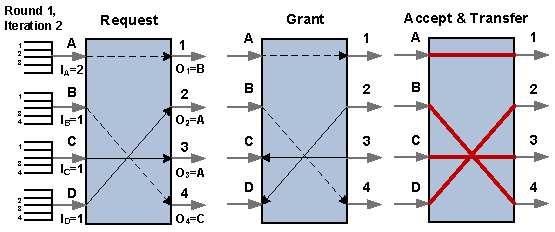
\includegraphics[width=1\linewidth]{algoritmus_islip_priklad_2.pdf}
    \caption{Příklad činnosti algoritmu iSLIP, kolo 2.}
\end{figure}

\begin{figure}[H]
    \centering
    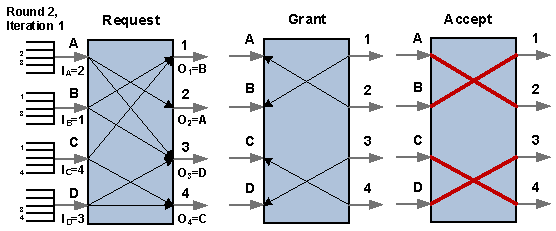
\includegraphics[width=1\linewidth]{algoritmus_islip_priklad_3.pdf}
    \caption{Příklad činnosti algoritmu iSLIP, kolo 3.}
\end{figure}

%%%%%%%%%%%%%%%%%%%%%%%%%%%%%%%%%%%%%%%%%%%%%%%%%%%%%%%%%%%%%%%%%%%%%%%%%%%%%%%%

\section{Přepínače s přepínanou propojovací deskou: vícestupňové přepínání}

Vlastnosti jednostupňového křížového přepínače:
\begin{compactitem}
    \item S počtem portů roste kvadraticky velikost přepínacího pole.
    \item Vnitřní blokování (soupeření o porty).
    \item Blokování na začátku fronty (\textit{head of line blocking}).
    \item Součástí přepínání je hledání maximálního párování.
\end{compactitem}

\noindent Je možné zvětšit počet portů, aniž by se dramaticky rozšířila velikost přepínacího pole? Ano, pomocí vícestupňového přepínání (vstup $\rightarrow$ vnitřní přepínací obvody $\rightarrow$ výstup).
\begin{compactitem}
    \item Nemají vnitřní blokování~--~Nejsou potřeba plánovací algoritmy pro hledání maximálního párování.
\end{compactitem}

\subsection{Přepínací síť Clos}

$Clos(m, n, r)$
\begin{compactitem}
    \item $r$ vstupních bloků s $n$ vstupy (bloků = křížový přepínač)
    \item $r$ výstupních bloků s $n$ vstupy
    \item $m$ vnitřních bloků s $r$ vstupy
\end{compactitem}

\noindent Closův teorém: \begin{compactitem}
    \item Pokud $m \geq 2n - 1$, pak lze přidat nové propojení vstupu a výstupu bez přeskládání (síť je neblokující). \begin{compactitem}
        \item Pokud všechny požadavky na vstupu jdou na jiné výstupy, pak pro jakoukoliv konfiguraci vstupů a výstupů je síť neblokující (pokud nejdou dva vstupy na jeden stejný výstup).
    \end{compactitem}
\end{compactitem}

\begin{figure}[H]
    \centering
    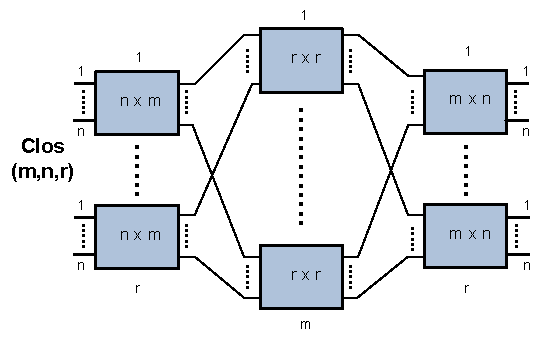
\includegraphics[width=0.75\linewidth]{clos.pdf}
    \caption{Obecné schéma Closovy sítě.}
\end{figure}

\begin{figure}[H]
    \centering
    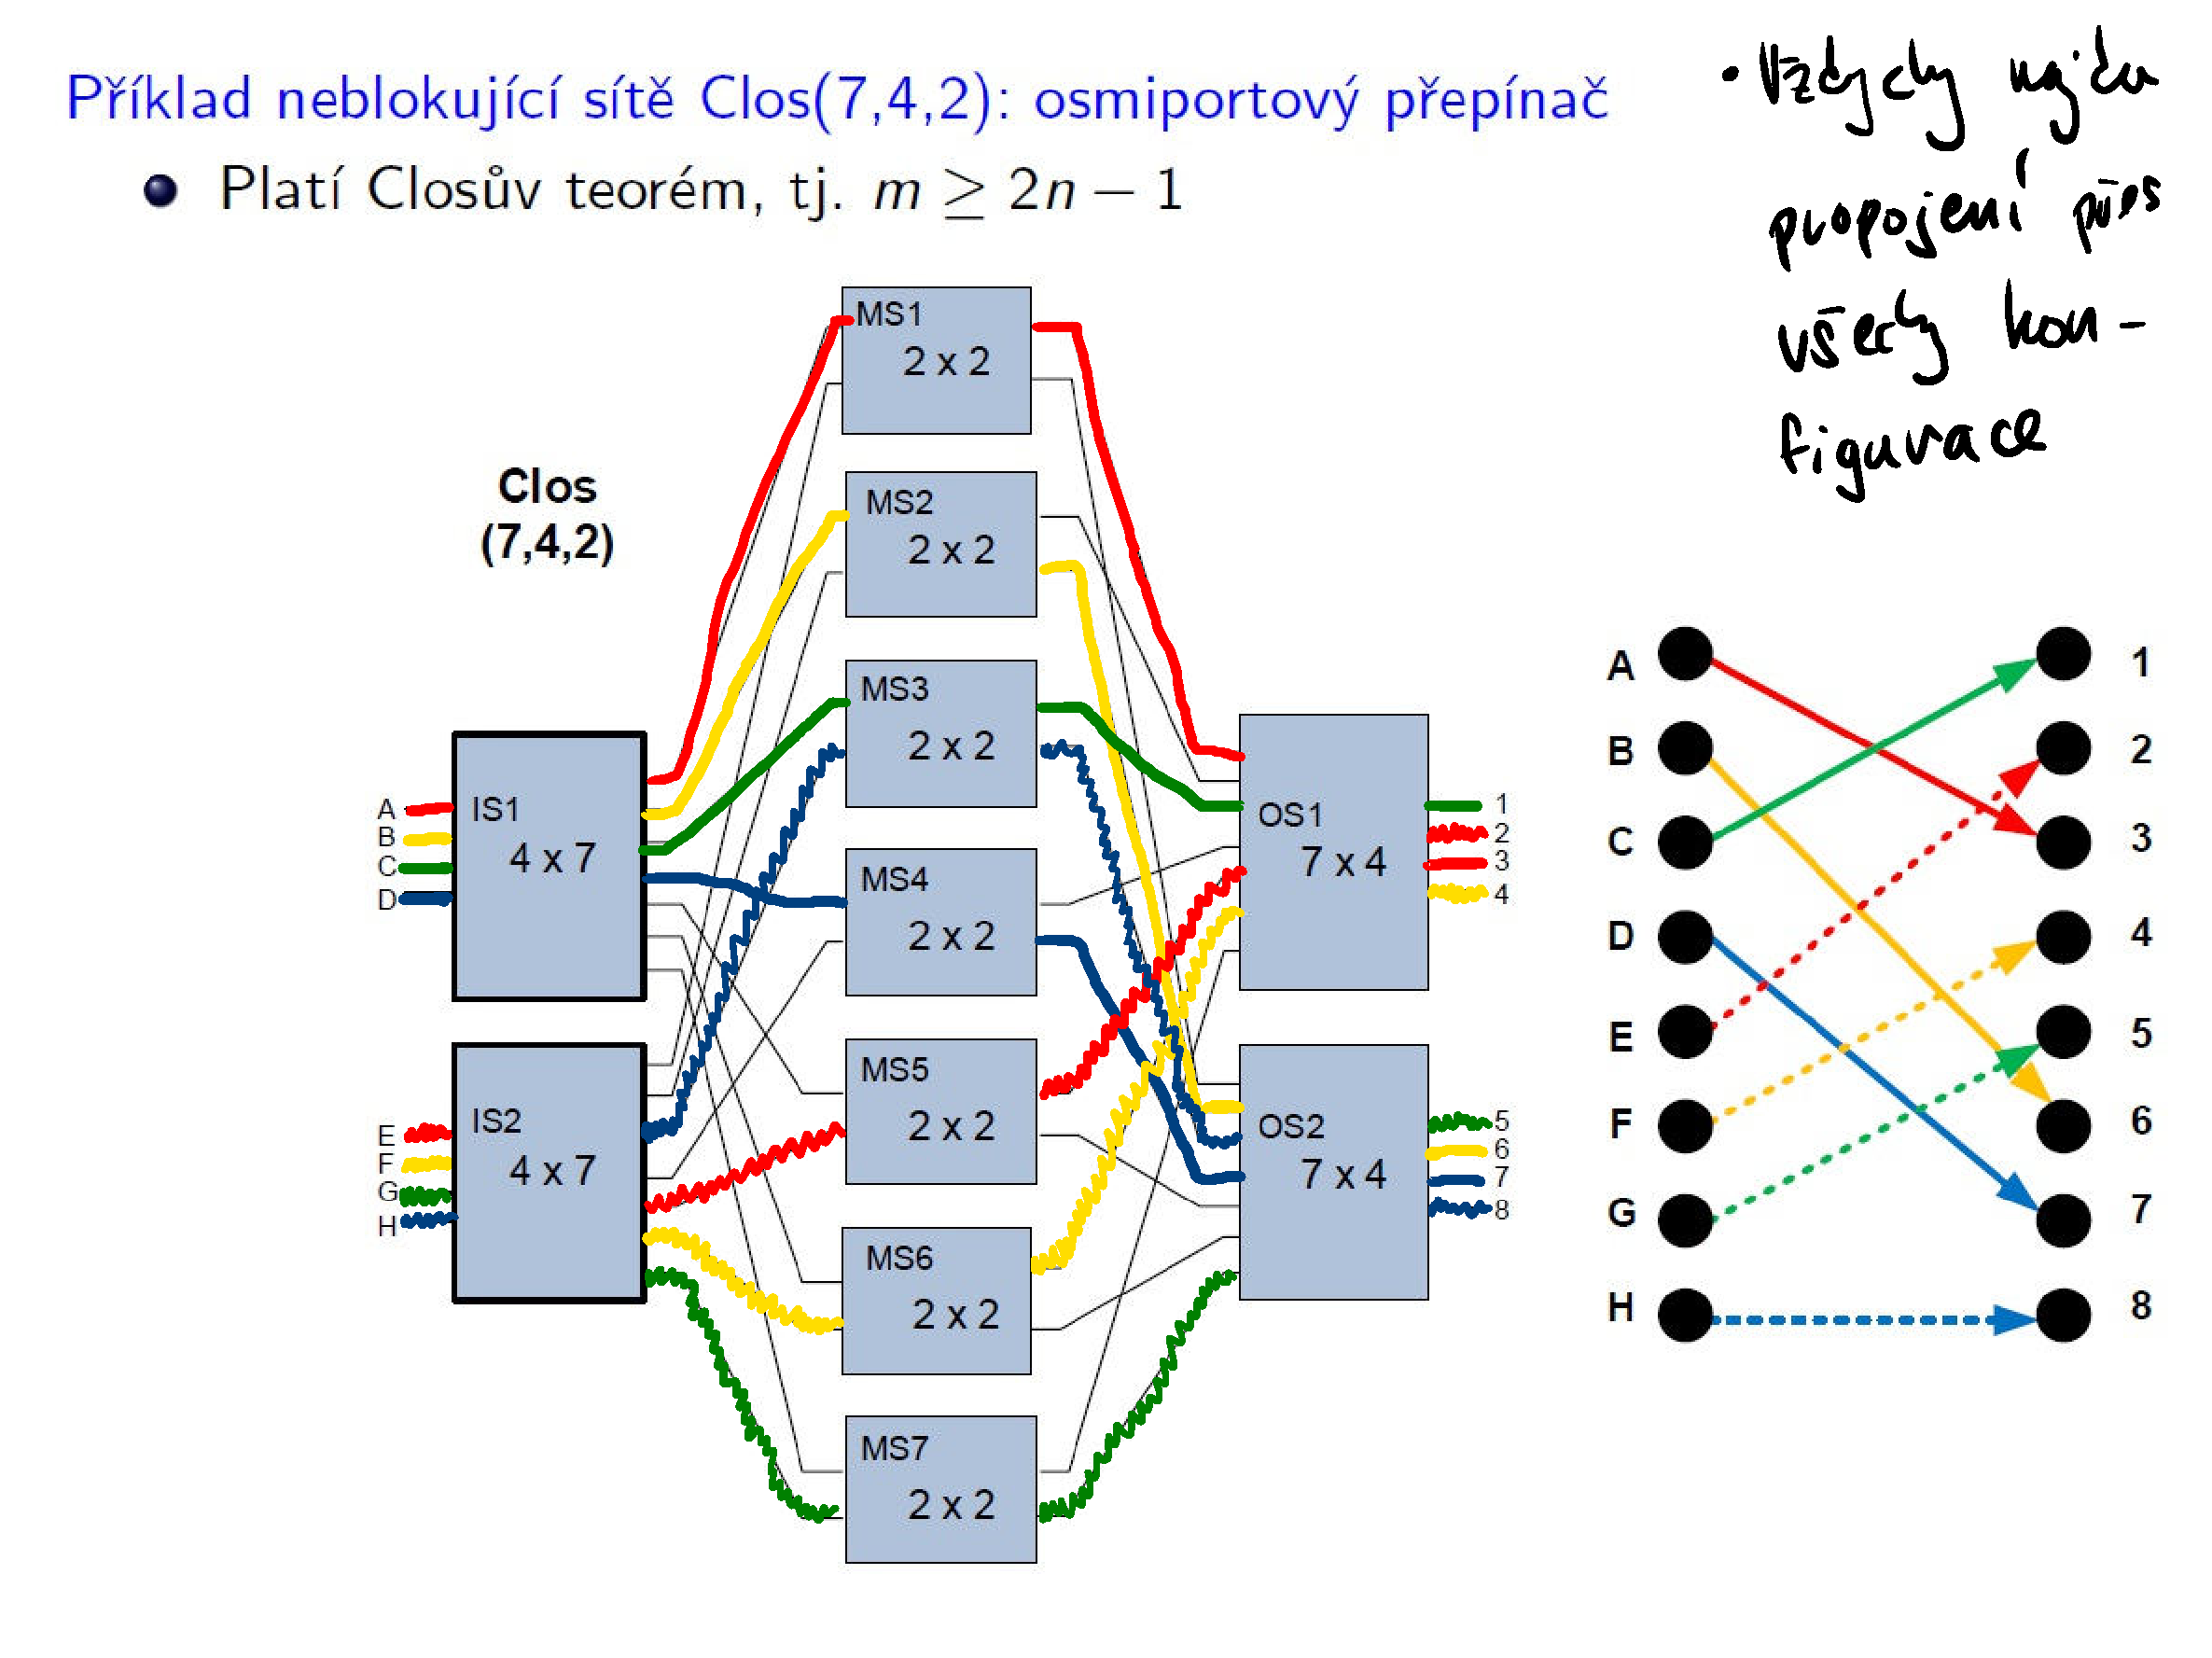
\includegraphics[width=1\linewidth]{clos_priklad.pdf}
    \caption{Příklad Closovy sítě.}
\end{figure}

\subsection{Modifikovaná přepínací síť Clos}

\begin{compactitem}
    \item Pokud $m \geq n$, pak je síť neblokující po přeskládání.
    \item Výpočetní složitost přeskládání je $O(N \log{D})$, kde $D$ je počet barev.
    \item Proč? Při plnění closova teorému je potřeba hodně bloků. Při této podmínce stačí výrazně méně a složitost výpočtu přeskládání je přijatelná.
\end{compactitem}

\begin{figure}[H]
    \centering
    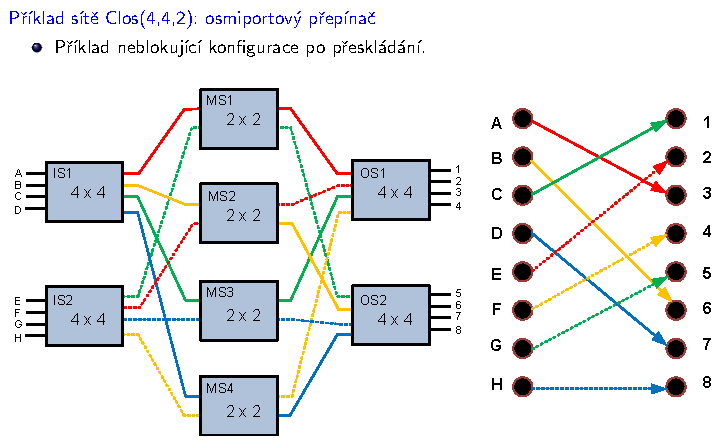
\includegraphics[width=1\linewidth]{clos_modifikovany_priklad.pdf}
    \caption{Příklad modifikované Closovy sítě.}
\end{figure}

\subsection{Přepínací síť Beneš}

$Benes(n)$ také $BN(n)$
\begin{compactitem}
    \item Základem je modifikovaná síť $Clos(m=2, n=2, r=1)$.
    \item Rekurzivní konstrukce sítě $Benes(n)$, kde $n$ je stupeň rekurze.
    \item Vstupní a výstupní přepínače velikosti $2 \times 2$.
    \item Celkový počet vstupních/výstupních portů $N = 2^n$.
    \item Prostřední část rekurzivních bloků $BN(n-1)$.
    \item Neblokující po přeskládání~--~algoritmus hledání propojení (žádné soupeření o vnitřní uzly nebo výstupní porty).
\end{compactitem}

\begin{figure}[H]
    \centering
    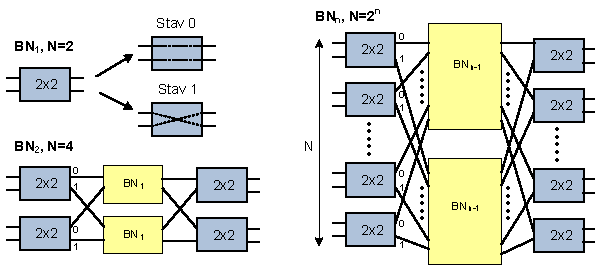
\includegraphics[width=0.9\linewidth]{benes.pdf}
    \caption{Obecné schéma Benešovy sítě.}
\end{figure}

\begin{figure}[H]
    \centering
    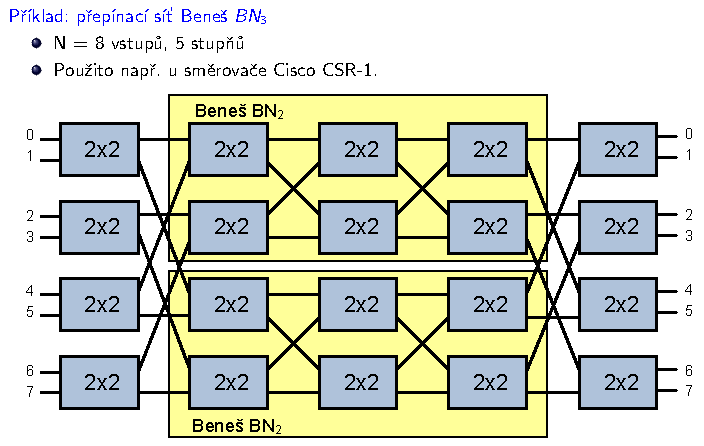
\includegraphics[width=0.9\linewidth]{benes_priklad_1.pdf}
    \caption{Příklad Benešovy sítě.}
\end{figure}

\begin{figure}[H]
    \centering
    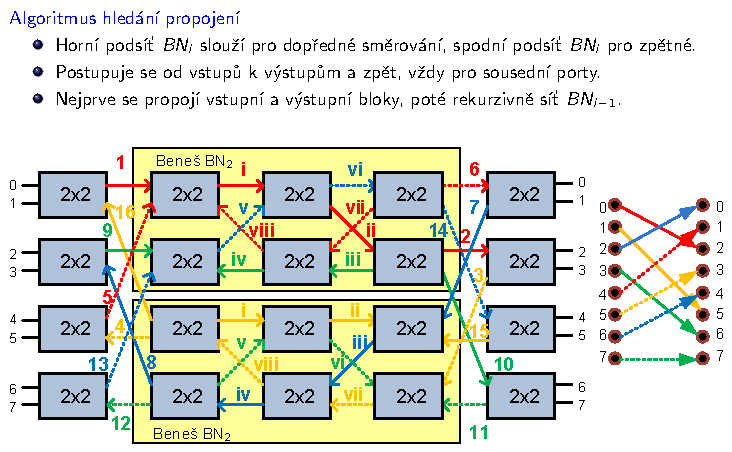
\includegraphics[width=1\linewidth]{benes_priklad_2.pdf}
    \caption{Příklad Benešovy sítě s přeskládáním.}
\end{figure}
